\documentclass{beamer}

\usepackage{graphicx}
\usepackage{hyperref}
\usepackage{amsmath}
\usepackage{svg}

\graphicspath{{./assets/}}

\usetheme{Rochester}

\hypersetup{
    colorlinks=true,
    linkcolor=blue,
    filecolor=magenta,      
    urlcolor=cyan,
    pdftitle={Presentation},
    pdfpagemode=FullScreen,
}

\title{H550 project defence}
\subtitle{Exploitation of an old access point}
\author{Aguililla Klein Esteban}
\institute{ULB}
\date{2024}

\begin{document}

\frame{\titlepage}

\begin{frame}
	\frametitle{Context}
	\begin{columns}
		\column{0.5\textwidth}
		\begin{itemize}
			\item released in october 2008
			\item end of sale in 2014
			\item end of support in 2019
			\item aimed at small businesses
		\end{itemize}
		\column{0.5\textwidth}
		\begin{figure}
			\centering	
			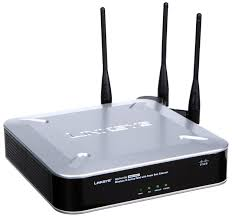
\includegraphics[width=\linewidth]{AP.jpg}
			\caption{WAP4410N Access Point}
		\end{figure}
	\end{columns}
\end{frame}
\begin{frame}
	\frametitle{lab setup}	
	\begin{figure}
		\centering	
		\scalebox{0.6}{
		\includesvg[scale=0.4]{assets/lab.svg}
		}
	\end{figure}
	\begin{itemize}
		\item local network without access to the internet
		\item the router is out of scope
	\end{itemize}
\end{frame}

\begin{frame}
	\frametitle{reconnaissance}
	\begin{columns}
		\column{0.5\textwidth}
		split into four parts, 
		\begin{enumerate}
			\item physical
			\item bootloader
			\item console
			\item network traffic
		\end{enumerate}
		\column{0.5\textwidth}
		\begin{itemize}
			\item architecture : 
				\begin{itemize}
					\item MIPS32
					\item big endian
				\end{itemize}
			\item memory :
				\begin{itemize}
					\item 48 TSOP NAND flash
					\item \href{https://www.alldatasheet.com/datasheet-pdf/view/267962/MCNIX/MX29LV640DBTC-90G.html}{MXIC-29LV640DBTC}
				\end{itemize}
			\item I/O :
				\begin{itemize}
					\item UART 3.3V
				\end{itemize}
		\end{itemize}
	\end{columns}
\end{frame}

\begin{frame}
	\frametitle{finding the uart}
	\begin{columns}
		\column{0.7\textwidth}	
		to find the UART, take measures with a multimeter
		\begin{center}
		\begin{tabular}{|c|c|c|c|}
			\hline
			pin & $R_{VSS}$ & $V$ & info \\ 
			\hline
			1 & $8.6k\Omega$ & $\approx 3.3V & VCC \\
			2 & $\infty k\Omega$ & $\approx 0V$ & TX\\
			3 & $\infty k\Omega$ & $\approx 0V - VCC$ & RX \\
			4 & $0 k \Omega$ & $0V$ & GND \\
			\hline
		\end{tabular}
		\end{center}
		in some cases it might be disabled, broken, \dots
		\column{0.3\textwidth}	
		\begin{fiure}
			\centering	
			\scalebox{0.5}{
			\includesvg[scale=0.5,angle=90]{assets/uart.svg}
		}
		\end{fiure}
	\end{columns}
\end{frame}

\begin{frame}[fragile]
	\frametitle{bootloader}	
	after connecting to the uart,
	\begin{itemize}
		\item boot log (a lot of useful information)
		\item can interrupt autoboot and get to U-boot console
	\end{itemize}
	in the U-boot console,
	\begin{itemize}
		\item unprotected
		\item reduced subset of U-boot (or is it due to the age ?)
		\item info about the hw, firmware, \alert{memory layout}
	\end{itemize}
	\begin{verbatim}
	ar7100> bdinfo
	flashstart  = 0xBF000000
	flashsize   = 0x00800000
	flashoffset = 0x0002F690
	\end{verbatim}
\end{frame}

\begin{frame}[fragile]
	\frametitle{console}
	\begin{columns}
		\column{0.3\textwidth}	
		\begin{itemize}
			\item ash shell
			\item busybox
				\begin{itemize}
					\item old version
					\item reduced
				\end{itemize}
			\item root user
			\item squashfs3
				\begin{itemize}
					\item readonly	
				\end{itemize}
			\item utilities for handling the device internals

		\end{itemize}
		\column{0.7\textwidth}
		extracting the partition table,
		\begin{verbatim}
[VAP0 @ wap86eb04]# cat /proc/mtd    
dev:    size   erasesize  name  
mtd0: 00040000 00010000 "u-boot"  
mtd1: 00010000 00010000 "u-boot-env"  
mtd2: 00650000 00010000 "rootfs"  
mtd3: 00140000 00010000 "uImage"  
mtd4: 00010000 00010000 "nvram"  
mtd5: 00010000 00010000 "calibration"	
		\end{verbatim}
		firmaware version,
	\end{columns}
\end{frame}

\begin{frame}
	\frametitle{network}
	something todo	
\end{frame}

\end{document}
